
%% bare_conf.tex
%% V1.3
%% 2007/01/11
%% by Michael Shell
%% See:
%% http://www.michaelshell.org/
%% for current contact information.
%%
%% This is a skeleton file demonstrating the use of IEEEtran.cls
%% (requires IEEEtran.cls version 1.7 or later) with an IEEE conference paper.
%%
%% Support sites:
%% http://www.michaelshell.org/tex/ieeetran/
%% http://www.ctan.org/tex-archive/macros/latex/contrib/IEEEtran/
%% and
%% http://www.ieee.org/

%%*************************************************************************
%% Legal Notice:
%% This code is offered as-is without any warranty either expressed or
%% implied; without even the implied warranty of MERCHANTABILITY or
%% FITNESS FOR A PARTICULAR PURPOSE!
%% User assumes all risk.
%% In no event shall IEEE or any contributor to this code be liable for
%% any damages or losses, including, but not limited to, incidental,
%% consequential, or any other damages, resulting from the use or misuse
%% of any information contained here.
%%
%% All comments are the opinions of their respective authors and are not
%% necessarily endorsed by the IEEE.
%%
%% This work is distributed under the LaTeX Project Public License (LPPL)
%% ( http://www.latex-project.org/ ) version 1.3, and may be freely used,
%% distributed and modified. A copy of the LPPL, version 1.3, is included
%% in the base LaTeX documentation of all distributions of LaTeX released
%% 2003/12/01 or later.
%% Retain all contribution notices and credits.
%% ** Modified files should be clearly indicated as such, including  **
%% ** renaming them and changing author support contact information. **
%%
%% File list of work: IEEEtran.cls, IEEEtran_HOWTO.pdf, bare_adv.tex,
%%                    bare_conf.tex, bare_jrnl.tex, bare_jrnl_compsoc.tex
%%*************************************************************************

% *** Authors should verify (and, if needed, correct) their LaTeX system  ***
% *** with the testflow diagnostic prior to trusting their LaTeX platform ***
% *** with production work. IEEE's font choices can trigger bugs that do  ***
% *** not appear when using other class files.                            ***
% The testflow support page is at:
% http://www.michaelshell.org/tex/testflow/



% Note that the a4paper option is mainly intended so that authors in
% countries using A4 can easily print to A4 and see how their papers will
% look in print - the typesetting of the document will not typically be
% affected with changes in paper size (but the bottom and side margins will).
% Use the testflow package mentioned above to verify correct handling of
% both paper sizes by the user's LaTeX system.
%
% Also note that the "draftcls" or "draftclsnofoot", not "draft", option
% should be used if it is desired that the figures are to be displayed in
% draft mode.
%
\documentclass[10pt, conference, compsocconf]{IEEEtran}
% Add the compsocconf option for Computer Society conferences.
%
% If IEEEtran.cls has not been installed into the LaTeX system files,
% manually specify the path to it like:
% \documentclass[conference]{../sty/IEEEtran}





% Some very useful LaTeX packages include:
% (uncomment the ones you want to load)


% *** MISC UTILITY PACKAGES ***
%
%\usepackage{ifpdf}
% Heiko Oberdiek's ifpdf.sty is very useful if you need conditional
% compilation based on whether the output is pdf or dvi.
% usage:
% \ifpdf
%   % pdf code
% \else
%   % dvi code
% \fi
% The latest version of ifpdf.sty can be obtained from:
% http://www.ctan.org/tex-archive/macros/latex/contrib/oberdiek/
% Also, note that IEEEtran.cls V1.7 and later provides a builtin
% \ifCLASSINFOpdf conditional that works the same way.
% When switching from latex to pdflatex and vice-versa, the compiler may
% have to be run twice to clear warning/error messages.






% *** CITATION PACKAGES ***
%
%\usepackage{cite}
% cite.sty was written by Donald Arseneau
% V1.6 and later of IEEEtran pre-defines the format of the cite.sty package
% \cite{} output to follow that of IEEE. Loading the cite package will
% result in citation numbers being automatically sorted and properly
% "compressed/ranged". e.g., [1], [9], [2], [7], [5], [6] without using
% cite.sty will become [1], [2], [5]--[7], [9] using cite.sty. cite.sty's
% \cite will automatically add leading space, if needed. Use cite.sty's
% noadjust option (cite.sty V3.8 and later) if you want to turn this off.
% cite.sty is already installed on most LaTeX systems. Be sure and use
% version 4.0 (2003-05-27) and later if using hyperref.sty. cite.sty does
% not currently provide for hyperlinked citations.
% The latest version can be obtained at:
% http://www.ctan.org/tex-archive/macros/latex/contrib/cite/
% The documentation is contained in the cite.sty file itself.






% *** GRAPHICS RELATED PACKAGES ***
%
\ifCLASSINFOpdf
  % \usepackage[pdftex]{graphicx}
  % declare the path(s) where your graphic files are
  % \graphicspath{{../pdf/}{../jpeg/}}
  % and their extensions so you won't have to specify these with
  % every instance of \includegraphics
  % \DeclareGraphicsExtensions{.pdf,.jpeg,.png}
\else
  % or other class option (dvipsone, dvipdf, if not using dvips). graphicx
  % will default to the driver specified in the system graphics.cfg if no
  % driver is specified.
  % \usepackage[dvips]{graphicx}
  % declare the path(s) where your graphic files are
  % \graphicspath{{../eps/}}
  % and their extensions so you won't have to specify these with
  % every instance of \includegraphics
  % \DeclareGraphicsExtensions{.eps}
\fi
% graphicx was written by David Carlisle and Sebastian Rahtz. It is
% required if you want graphics, photos, etc. graphicx.sty is already
% installed on most LaTeX systems. The latest version and documentation can
% be obtained at:
% http://www.ctan.org/tex-archive/macros/latex/required/graphics/
% Another good source of documentation is "Using Imported Graphics in
% LaTeX2e" by Keith Reckdahl which can be found as epslatex.ps or
% epslatex.pdf at: http://www.ctan.org/tex-archive/info/
%
% latex, and pdflatex in dvi mode, support graphics in encapsulated
% postscript (.eps) format. pdflatex in pdf mode supports graphics
% in .pdf, .jpeg, .png and .mps (metapost) formats. Users should ensure
% that all non-photo figures use a vector format (.eps, .pdf, .mps) and
% not a bitmapped formats (.jpeg, .png). IEEE frowns on bitmapped formats
% which can result in "jaggedy"/blurry rendering of lines and letters as
% well as large increases in file sizes.
%
% You can find documentation about the pdfTeX application at:
% http://www.tug.org/applications/pdftex





% *** MATH PACKAGES ***
%

\usepackage[cmex10]{amsmath}
\usepackage{tikz}

\definecolor{bluekeywords}{rgb}{0,0,1}
\definecolor{greencomments}{rgb}{0,0.5,0}
\definecolor{redstrings}{rgb}{0.64,0.08,0.08}
\definecolor{xmlcomments}{rgb}{0.5,0.5,0.5}
\definecolor{types}{rgb}{0.17,0.57,0.68}

\usepackage{listings}

\usepackage[]{algorithm}
\usepackage{algorithmic}
\usepackage{subcaption}
\usepackage{etoolbox}
\usepackage{minted}
\usepackage{color}
\definecolor{LightGray}{rgb}{0.9, 0.9, 0.9}
\usepackage{verbatim}
\usepackage{caption}
\usepackage{mdframed}
\usepackage{stmaryrd}			% for \llbracket symbols [[ ]]
\usepackage{amsmath, amssymb}
\usepackage{multirow}
\newcommand{\iseg}[1]{{\left\llbracket #1 \right\rrbracket}} % integer segment
\newcommand{\nset}{\mathbb{N}}
\newcommand{\zset}{\mathbb{Z}}
\newcommand{\rset}{\mathbb{R}}
\newcommand{\cset}{\mathbb{C}}
\newcommand{\qset}{\mathbb{Q}}

\newcommand{\algorithmicdoinparallel}{\textbf{do in parallel}}
\makeatletter
\AtBeginEnvironment{algorithmic}{%
  \newcommand{\FORALLP}[2][default]{\ALC@it\algorithmicforall\ #2\ %
    \algorithmicdoinparallel\ALC@com{#1}\begin{ALC@for}}%
}
\makeatother


% correct bad hyphenation here
\hyphenation{op-tical net-works semi-conduc-tor}

\newtheorem{theorem}{Theorem}[section]
\newtheorem{lemma}[theorem]{Lemma}
\newtheorem{proposition}[theorem]{Proposition}
\newtheorem{corollary}[theorem]{Corollary}
\newtheorem{property}[theorem]{Property}
\newtheorem{definition}[theorem]{Definition}
\newtheorem{remark}[theorem]{Remark}
\newtheorem{assumption}[theorem]{Assumption}

\newcommand{\norm}[1]{\left\lVert#1\right\rVert}


\begin{document}
%
% paper title
% can use linebreaks \\ within to get better formatting as desired
\title{Distributed and in-Situ machine learning for smart-homes and buildings: application to alarm sounds detection}


% author names and affiliations
% use a multiple column layout for up to two different
% affiliations

\author{\IEEEauthorblockN{Amaury Durand}
\IEEEauthorblockA{Telecom ParisTech\\
Paris, France\\
amaury.durand@telecom-paristech.fr}
\and
\IEEEauthorblockN{Yanik Ngoko}
\IEEEauthorblockA{Qarnot Computing and University of Paris 13\\
Paris, France\\
yanik.ngoko@qarnot-computing.com}
\and
\IEEEauthorblockN{Christophe C\'erin}
\IEEEauthorblockA{University of Paris 13\\
Paris, France\\
christophe.cerin@lipn.univ-paris13.fr}
}

\maketitle

\setlength{\abovecaptionskip}{0pt}
\setlength{\belowcaptionskip}{0pt}
\setlength{\intextsep}{1pt}
\setlength{\dbltextfloatsep}{3pt}
\setlength{\textfloatsep}{3pt}


\begin{abstract}
The need to build real-time, context-aware, secure and intelligent systems is pushing forward in-situ machine learning. 
In this paper, we consider the implementation of such systems with the computing model promoted by 
Qarnot computing. Qarnot introduced an utility computing model in which servers are distributed in homes and offices where they
serve as heaters. The Qarnot servers also embed several sensors that, in the environment in which they are deployed, are able to continuously 
collect diverse data related for instance to the temperature, humidity, $\mathbf{CO_2}$ etc. The goal of our paper is to show how, 
in the Qarnot platform, one can develop distributed and in-situ workflows for {\it smart-homes problems}. For this, 
we consider a typical problem: the detection of alarm sounds. Our paper introduces a new orchestration system for in-situ workflows, 
in the Qarnot platform. 
The specificity of this system is to be based on the software development kit and the scheduler of the Qarnot platform.
We also consider a general parallel framework for training alarm sound classifiers and decline an implementation that makes 
use of our orchestrator.
The implemented framework is next evaluated on different aspects including: the accuracy (of the resulting classifiers), the granularity of parallelism and the scalability of the implementation. The results we obtain are encouraging, they comfort the idea that the Qarnot model is certainly one of the most effective platforms for distributed and in-situ machine learning. 
\end{abstract}

\begin{IEEEkeywords}
in-situ machine learning; distributed machine-learning; alarm sounds detection;  performance evaluation

\end{IEEEkeywords}


% For peer review papers, you can put extra information on the cover
% page as needed:
% \ifCLASSOPTIONpeerreview
% \begin{center} \bfseries EDICS Category: 3-BBND \end{center}
% \fi
%
% For peerreview papers, this IEEEtran command inserts a page break and
% creates the second title. It will be ignored for other modes.
\IEEEpeerreviewmaketitle


\section{Introduction} \label{Introduction}

The question of the adequate architecture for the Internet of Things (IoT) has always been a main concern. At the first age of the 
IoT revolution, this questioning led to the development of huge datacenters that integrate machine learning and Big Data systems. 
However, this initial model showed several important limitations on privacy, Internet congestion, 
response time~\cite{DBLP:conf/lcn/Roelands13}. As an alternative, several works propose to decentralize this original IoT model by deporting the IoT logic of traditional clouds into edge clouds or embedded systems that serve for computing the intelligence of a smart environment (home, building, city etc.). For machine learning, 
this direction promotes {\it in-situ} solutions where one of the main challenge is to deploy complex machine learning 
workloads into {\it modest} computing platforms available in homes, offices etc. In this paper, we are interested in building distributed machine learning 
systems that are able to locally train and improve models from homes or buildings in which their sensory data is issued. 
Our paper discusses such a system in considering the utility computing model introduced by 
Qarnot computing. 

	\begin{figure*}[htbp]
          \begin{subfigure}[b]{0.4\textwidth}
            \centering
            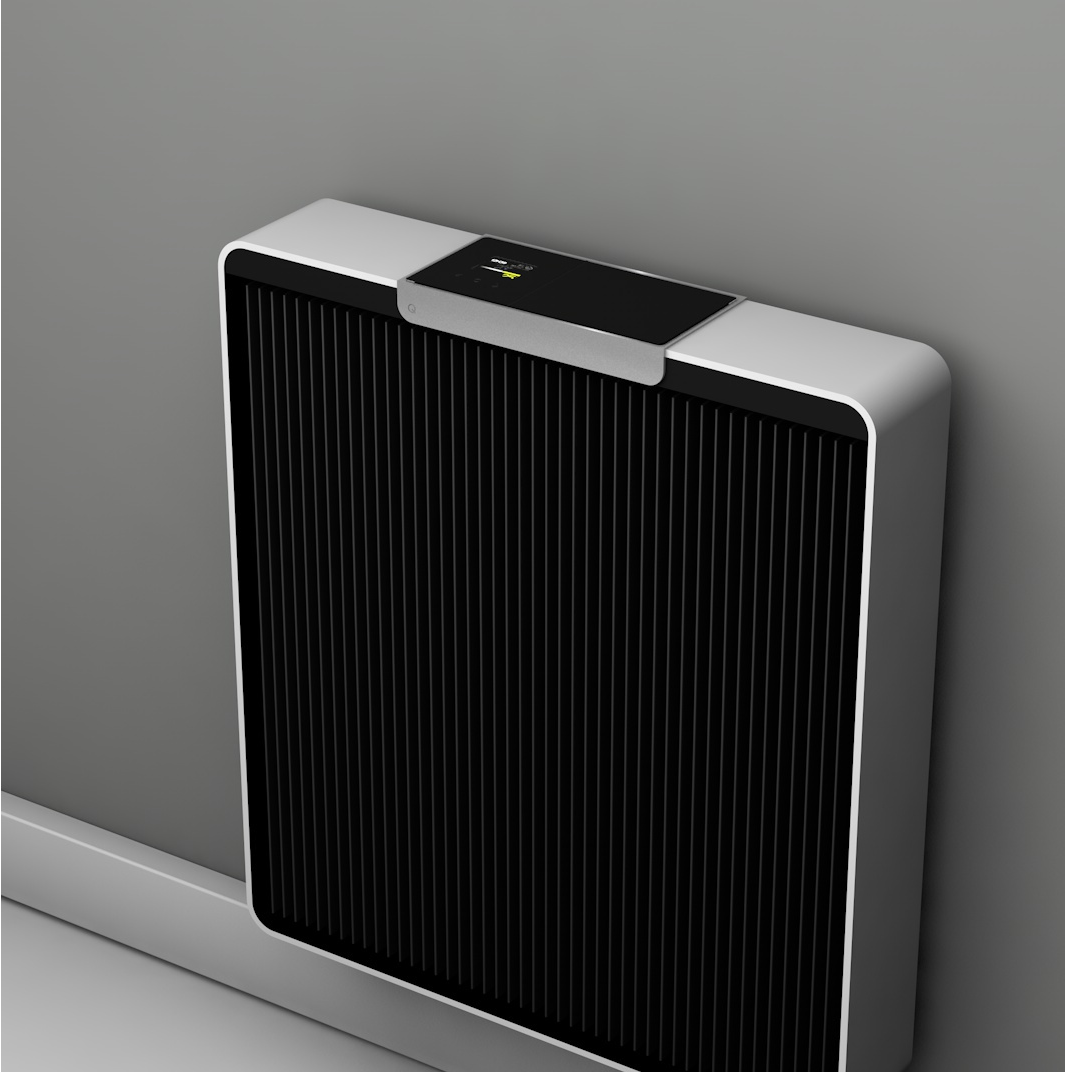
\includegraphics[width=4cm,height=3.5cm]{./Figures/rad.png}
            \caption{\scriptsize A Q.rad }
          \end{subfigure}
          \begin{subfigure}[b]{0.4\textwidth}
            \centering
            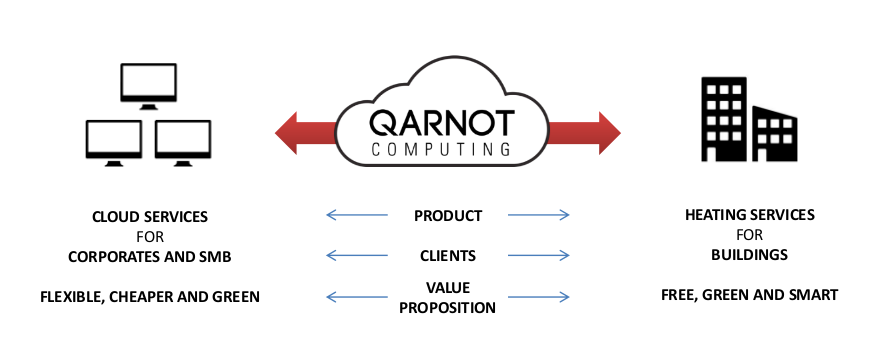
\includegraphics[width=10.7cm,height=3.5cm]{./Figures/model.png}
            \caption{\scriptsize The roles of the Q.ware }
          \end{subfigure}
	\caption{The Qarnot model}
	\label{fig:digital}
	\end{figure*}


Qarnot computing~\footnote{www.qarnot-computing.com} promotes a cloud computing model where heating, computing, 
storage and networking is provided from a single infrastructure: a network of geo-distributed servers deployed in homes, offices and buildings. 
The Qarnot model is based on two main products. The first is a new model of servers (Q.rads) in which the cooling system is replaced by a 
heat diffusion system, regulated by a thermostat. Each Q.rad (See Figure~\ref{fig:digital}) embeds several processors in addition to sensors 
related to humidity, $\mathrm{CO_2}$, presence etc. The second Qarnot product is a new middleware (Q.ware) for on-demand computing. Q.ware manages 
two types of requests: requests for processing cloud services and requests for heating. Its goal is to deploy and 
adjust the run of cloud workloads to meet the heat demand on Q.rads. For more details about the Qarnot model, we refer the interested 
reader to~\cite{DBLP:conf/europar/Ngoko16}.

Considering data or processes, the Qarnot model is appropriate for in-situ machine learning. Indeed, in the data viewpoint, 
its sensing capacities can be used to create local datasets for machine problems to solve at the scale of a home or building. 
The Qarnot platform supports a data service (QaIoT) that collects sensory data in Q.rads 
and make them available to programs designed for Q.rads. 
In the viewpoint of processes, the distributed learning processes can be performed in the home or building for which we want to 
build a learning system. The Qarnot platform includes a software development kit (SDK) for building local orchestrations 
of processes in homes, buildings or cities.
The global objective of this paper is to show how with these two tools (QaIoT and the Qarnot SDK), 
one can develop complex in-situ machine learning workflows for problems related to smart-homes and buildings. 
We focus on the construction of alarm sound classifiers.  Indeed, the behavior of an alarm sound classifier will be impacted by the 
difference between the background noises, used in its construction, and the natural sound flow in which it operates. 

Our paper makes three important contributions. Firstly, we introduce a general orchestration system for implementing in-situ 
distributed learning frameworks and in particular, a solution for the alarm sounds detection, with the Qarnot SDK. 
The orchestration system includes an API and a scheduler. 
The API of the orchestration system is based on abstractions close to the one used in 
GraphLab~\cite{Low:2012:DGF:2212351.2212354} (data model and update functions) and the concept of {\it Processors} used 
in the \texttt{madmom} library \cite{DBLP:journals/corr/BockKSKW16}. However, the abstractions are adjusted to fit with the 
object oriented interface of the Qarnot SDK. Differently from the Qarnot SDK, the orchestrator API includes simple 
constructs for the description of workflows. 

The alarm detection framework we use for validating the orchestrator is based on energy, spectral and Mel-frequency cepstral features~\cite{ganchev2005comparative}, \cite{pyAudioAnalysis}
and a Pareto-selection method for choosing the best classifiers. We consider three techniques for building classifiers: the support vector machine (SVM), the logistic regression and the K-Nearest Neighbour (KNN). Our second contribution is to propose a possible parallel 
implementation for training the alarm framework based on the orchestrator. Finally, we explore this implementation and evaluate its accuracy, 
false and true positive rate and runtime performance. We discuss the best granularity (from coarse-grained to fine-grained) and the scalability of the proposed implementation.

The rest of the paper is organized as follows. In Section~\ref{Related}, we present the related works. 
In Section~\ref{Framework}, we discuss of the acoustic alarm detection framework that we consider. In Section~\ref{Model}, we describe 
the key services that the Qarnot platform offers for in-situ machine learning. In Section~\ref{Orchestrator}, we explain 
how we implement the training process of the framework that we introduced. A performance evaluation is done in 
Section~\ref{Proof-of-concept} and we conclude in Section~\ref{Conclusion}.

\section{Related work} \label{Related}

Our contribution is to put into perspective with the recent advances that led to the profusion of tools for parallel 
machine learning. Our work is also related to prior contributions in machine learning for acoustic alarm detection. 

Regarding recent parallel machine learning tools, we propose to distinguish between three main trends. 
The first trend includes the development of orchestrators for Big Data systems that are based on Hadoop~\footnote{http://hadoop.apache.org/} or related systems. 
In these solutions, the parallelism is generally formulated within the Map-reduce paradigm~\cite{DBLP:journals/cacm/DeanG10}. 
In the second trend, the restrictions of the Map-reduce paradigm are overcome using more general graph-based abstractions like 
the Directed Acyclic Graphs (DAG) (solutions that are related to the distributed GraphLab~\cite{Low:2012:DGF:2212351.2212354}).  Finally the last trend is related to the development of parallel systems for deep learning algorithms in which the key novelty is to exploit the parallelism at the GPU level~\cite{Raina:2009:LDU:1553374.1553486}.
Our proposition is neither based on Map-reduce, nor on GPUs. As already said, the orchestrator we introduce 
is based on an upper layer abstraction close to the one we can find in GraphLab. However, our conceptualization manipulates object 
oriented concepts of the Qarnot SDK. In addition, our solution is specially designed for in-situ learning. 

The field of supervised machine learning for audio classification (that includes alarm sound detection) is well-established. There is a large consensus on the class of features that are meaningful in this context~\cite{Mckinney03featuresfor,DBLP:journals/taslp/JoderER09} 
and some classification methods like the logistic regression has been successfully applied in several cases. It was also showed 
that for sound detection systems to work in the real-world, it is important to train the classifiers with 
background noises that are representative of the environment in which the classifiers will operate~\cite{DBLP:conf/icassp/SalamonB15}. 
In other words, {\it in-situ} and context-aware learning is welcome on the problem. 


Few works however dealt with the in-situ perspective of this work (collect and process data locally). The closer work we found is the 
Auditeur system~\cite{Nirjon:2013:AMS:2462456.2464446}. The system proposes a context-aware solution for acoustic events detection on smartphones. 
The Auditeur system is composed of: a phone client that captures, processes and can run a {\it classification plan} and a cloud 
service that, based on audio and contextual information sent by a phone, could generate an appropriate classification plan to be 
followed at the smartphone level. We did not investigate whether or not the workflow we propose could be applied 
to any acoustic event. The main difference between our work and Auditeur is that part of the processing could be done 
remotely with Auditeur while we propose to collect and process 
data in a same environment, which is more interesting for real-time and security.

\section{Training framework for alarm sound detection } \label{Framework}
\subsection{General problem}

We assume a home with a fire-alarm and a set of Q.rads. Each Q.rad embeds two microphones and can record the input audio 
stream. We also assume that the sound is recorded at a fixed \footnote{we use $44100Hz$} sample rate in a wav file. {\it The goal is to build  a detection system which, given any wav file of $T$ samples, could state whether or not it contains an alarm sound}.

The system to build has $3$ subsystems: a data collection system, a training system and a decision system. 
The data collection system creates the dataset of wav files that will be used for training and validation. 
From the training dataset, the training system is able to generate a subset of dominant classifiers. Assuming we have classifiers that are trained for each input audio, the decision system states whether or not the audio contains a fire-alarm sound.

Our paper mainly focuses on the training system. However, we will shortly discuss the data collection system in order 
to explain how we create training dataset in-situ.

\subsection{Data collection}

The challenging question here is to make sure that the data used to build the classifiers are representative of the environment 
in which the Q.rads are. Our proposition is to create the training and testing datasets in mixing known alarm sounds with 
background sounds of the environment for which we are building a classifier. More precisely, we assume that we have 
samples of the alarm sounds, we want to recognize. We also assume samples of significant sounds like a baby cry or a music. 
In these audio records (alarm and significant sounds), there is no background noise. The goal of the data collection 
system is to locally create from these sounds two datasets for training and evaluation where 
the background noises of the environment is introduced. This is summarized in Figure~\ref{fig:gen}. 
A challenge at this stage is to set-up some programmability rules for recording background noises. We must also decide on the date at which we consider that we have enough data for training. But due to space restriction, we will not discuss these details in this paper. However we will explain in Section~\ref{Model}, the 
system architecture that Qarnot proposes for data collection.

	\begin{figure}[hbtp]
	\begin{center}
	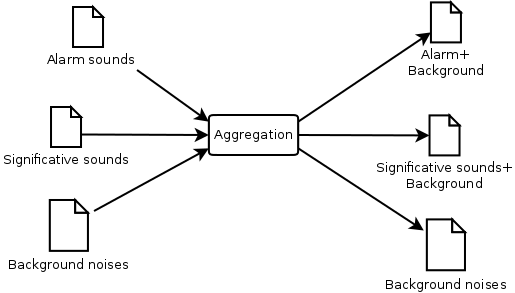
\includegraphics[scale=0.3]{./Figures/Aggregation.png}
	\caption{Automatic generation of the dataset: we mix alarm and significant sounds with the local background noises.}
	\label{fig:gen}
	\end{center}
	\end{figure}


\subsection{Training system}

In Figure~\ref{fig:training}, we illustrate the training framework we consider in our problem. The representation follows the 
BPMN notations (An empty lozenge is a join and a lozenge with a plus is a fork...). 

\begin{figure*}[htbp]
  \captionsetup{aboveskip=-5pt}
	\centering
	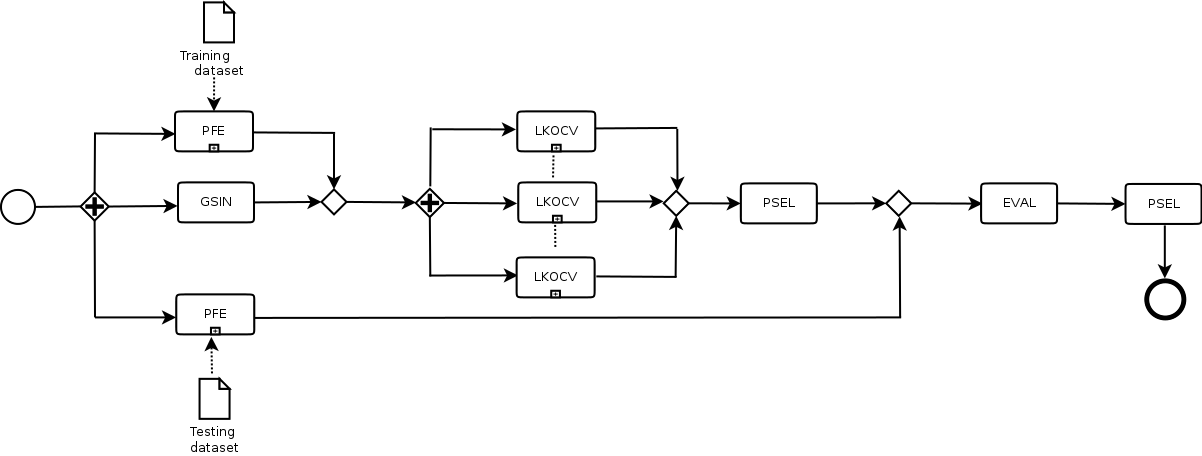
\includegraphics[scale=0.3]{./Figures/workflow.png}
	\caption{Training system}
	\label{fig:training}
	\end{figure*}

The framework is based on 5 activities and subprocesses that we discuss below.

\begin{itemize}

\item {\bf PFE:} Given a set of wav files, the goal here is to extract the acoustic features of the wav files. PFE is a subprocess 
consisting of a set of parallel activities where the acoustic features are separately computed from each dataset file. 
% The features we used are the classical ones used in signal processing (Mel-frequency spectrum~\cite{Davis:1990:CPR:108235.108239},energy etc.). Their complete list is defined in~\cite{pyAudioAnalysis}.

\item {\bf GSIN:} The framework implements a grid search process whose goal is to find the best classifiers depending on the 
parameters we use. GSIN consists in the initialization of this grid search. The goal is to generate the possible configurations 
we will explore. A configuration here includes: parameters related to features (discussed further) and hyper-parameters related to 
classification techniques (SVM, KNN ..).

\item {\bf LKOCV:} Given an input configuration (generated in GSIN), this subprocess starts with the run of a 
  time integration method whose goal is to refine the quality of information which training acoustic features provide by aggregating their values in time (see \ref{subsec:extraction} and \cite{DBLP:journals/taslp/JoderER09}). With the refined features, the next activity 
in the subprocess consists in building the classifier corresponding to the current configuration with a Leave-k-out cross-validation.
%Our learning techniques include: the SVM, logistic regression and KNN. 

\item {\bf PSEL:} From a list of classifiers whose False and True Positive rates (FPR, TPR) are defined (generated in LKOCV or EVAL), we select the ones that are in the Pareto front where we minimize the FPR and maximize the TPR.

\item {\bf EVAL:}  Assuming a list of classifiers and the input features of the testing dataset, we evaluate here the classifiers on the testing features. The TPR and FPR of each classifier are returned.

\item {\bf TRAIN:} We train the selected classifiers with all data from training and testing sets.
\end{itemize}

It is important to notice that some activities in the proposed framework are parallel and distributed. For instance, at the beginning, 
the PFE activities could be done in parallel. The LKOCV activities also are performed in parallel (each parallel instance deals  
with a configuration). In the next, we will discuss of the component of the Qarnot architecture for 
its implementation.

\section{Architecture and programming model} \label{Model}

In the viewpoint of data, the network of Q.rads at the scale of a city or building is a composition of clusters, each 
associated with a QaIoT server. A QaIoT server aggregates and manages the sensory data issued from the Q.rads to which it is 
connected. A program deployed on a connected device (or a Q.rad) can get access to these data. For this purpose, 
it must first register to the QaIoT server by sending an Http request where it declines: the nature of the device (Q.rad, 
raspberry etc.), the Id of the device, the role it intends to play (e.g: access to the audio stream of the cluster). If the 
request is accepted a websocket communication will be established between the device and QaIoT in order to service the data
to the applicant program. In our case, the communication will consist in servicing real-time data.
A view of the QaIoT data service is given in Figure~\ref{subfig:qaiot}. 
It is easy to notice that the mixer of Figure~\ref{fig:gen} can be implemented as an applicant program that request the audio streams  
related to a home and then {\it mixes} the data with a set of alarms and significant sounds.

In the processing viewpoint, the Qarnot SDK is based on three main concepts: the notions of task, 
disks and docker image. A task is an object oriented abstraction that refers to a 
docker container or a set of containers to deploy and run. A task is associated with a docker image defined in the 
parameter {\it constants["DOCKER\_REPO"]}. We can specify a set of input files for a task in defining a {\it resource disk}. 
Such a disk is defined in the list parameter {\it resources} of the task. 
A task has a name and can be composed by subtasks (or parallel instances).  
In these cases, the run of each subtask will cause the deployment of a docker image. The process run by a task is defined in 
assigning a command line to the parameter {\it constants['DOCKER\_CMD']}. The execution will assume that the input 
files are available from the resource disk and and will generate output files in a {\it results disk}.

	\begin{figure*}[ht]
          \begin{subfigure}[b]{0.4\textwidth}
            \captionsetup{skip=0pt}
            \centering
            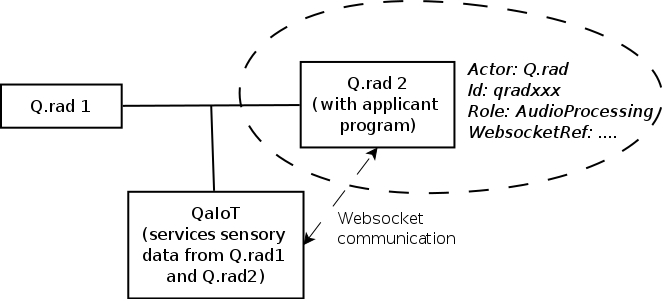
\includegraphics[scale=0.25]{./Figures/DataService.png}
            \caption{Data service \label{subfig:qaiot}}
          \end{subfigure}
          \begin{subfigure}[b]{0.6\textwidth}
            \captionsetup{skip=0pt}
            \centering
            \inputminted[baselinestretch=1, bgcolor=LightGray, fontsize=\scriptsize]{python}{sample.py}
            \caption{Example of scripts with the Qarnot SDK \label{subfig:sample}}
          \end{subfigure}
          \caption{Data service and Qarnot SDK example.} 
          \label{fig:arch}
	\end{figure*}

An example of script with the Qarnot SDK is proposed in Figure~\ref{fig:arch}. Finally, for in-situ learning, let us notice that 
in the way we define the constants of a task, we can indicate a specific Q.rad or a set of Q.rads on which we want the task to run.

\section{Orchestrating the alarm detection framework} \label{Orchestrator}
\subsection{The orchestrator API}
The orchestrator API relies on 2 basic concepts (implemented in \texttt{python}): 
\begin{itemize}
\item \textbf{QWork:} This represents a work to be done during the workflow. QWorks correspond to boxes in a diagram. They have 2 main attributes: \texttt{name} which enables to differentiate the QWorks and \texttt{nextname} which enables to define the next QWork in the workflow. A QWork also has a \texttt{process} method which represents the work to do. To make it even simpler, QWork instances are callable which means that they can be used as any function. 
\item \textbf{QData:} This represents the inputs and outputs of QWorks. A QData instance is a dictionary with 3 keys (it can be seen as a 3 columns table and we will keep this analogy for clarity): \texttt{data} (the actual data), \texttt{sender} (the name of the QWork which sends the data) and \texttt{receiver} (the name of the QWork which receives the data). 
\end{itemize}
These two concepts work together as follows (see algorithm \ref{alg:Qwork}): if \texttt{w} and \texttt{d} are respectively instances of QWork and QData, running \texttt{w(d)} makes \texttt{w} look for its \texttt{name} in \texttt{d}'s \texttt{receiver} column and process the corresponding row using the \texttt{process} method. In the \texttt{process} method, one can specify how to handle different \texttt{senders}.

Subclasses of QWork can then be defined to differentiate what is done locally and what is done in parallel using the Qarnot platform: 
\begin{itemize}
\item \textbf{QFunc:} a QFunc is a QWork which processes a particular function locally.
\item \textbf{QTask:} QTask inherits from QWork and Task (from the qarnot SDK). The QTask class has two particularities: 
the first one is that its input must be a disk (which will be added to the resources) or a serializable object (which will be put in a resource disk). This is done with a method called \texttt{add\_input\_to\_resources}. The second one is that there are two ways to run a QTask instance: \texttt{process} method (or calling the instance) which will submit the task and wait for it to be over, and the \texttt{submit} method which does not wait for the task to be over (which is useful for parallel tasks, see below). The output of a QTask is a results disk (as defined in the Qarnot SDK).
\end{itemize}
With these three tools (QData, QFunc, QTask) one could create basic parallel workflows composed of functions and tasks. To go a step further in the abstraction, we introduce two other subclasses of QWork that represent higher level concepts: 
\begin{itemize}
\item \textbf{QParallelWork:} A QParallelWork instance has a list of QWorks (except QTasks) and a list of QTasks and runs all of them in parallel using different threads (here QTasks and other QWorks were separated because we use the \texttt{submit} method for QTasks which does not exist in the others).
\item \textbf{QWorkflow:} This is the highest concept since it represents the workflow itself. A QWorkflow task has a list of QWorks and runs them in a {\it greedy} way which means that it only runs a QWork when its inputs are available (i.e when the previous QWork in the list stops).
\end{itemize}

To sum up, there are 4 subclasses of QWork: QFunc for basic functions, QTasks for tasks, QParallelWork for multithreading and QWorkflow to combine them all. QData makes the link between them.
By combining all these concepts, complex workflows can be implemented. Note that a QWorkflow can be put in a QParallelWork to run multiple workflows simultaneously. 
Algorithms \ref{alg:Qwork}, \ref{alg:Qtask}, \ref{alg:Qparallel}, \ref{alg:Qworkflow} sum up in pseudo-code the ways these concepts handle a given input. A QWork will call its \texttt{process} method. A QFunc's \texttt{process} method calls the function. A QTask will add the inputs to its resources and submit the task to the Q.Ware scheduler. A QParallelWork will submit all QTasks and run all other QWorks in different threads and then wait for all of them to finish. A QWorkflow will run all its QWorks.

Note that all QWorks which are not QTasks are processed locally, where the global QWorkflow is running, and all QTasks are submitted to the Q.Ware scheduler. In is important to precise that QTasks can be constrained to run in a specific Q.rad. Hence, our orchestrator manages two levels of scheduling: a local level where as soon as a Qwork can be done, it is processed or submitted to the Q.ware and the Q.ware level (external) where jobs are ran according to a FIFO (First In First Out) policy. Thus a QWorkflow can be strictly processed in a home.

In all the algorithms presented, QWorks need a QData as input, therefore if to handle multiple input one can either get inputs as different QData rows and differentiate them using the \texttt{sender} (see for example \texttt{f211} in figure \ref{fig:orch_ex}) or put a dictionary in the QData \texttt{data} column (see for example QCreateDisk below).

\begin{algorithm}[H]
\caption{QWork call method}
\label{alg:Qwork}
% \footnotesize
\small
\begin{algorithmic}
\REQUIRE \texttt{d} a QData instance
\ENSURE returns \texttt{d} without my input, with my output
\STATE find my name in \texttt{d["receiver"]}, remove the corresponding rows from \texttt{d} and put them in \texttt{d'}
\STATE out $\leftarrow$ \texttt{process}(\texttt{d'})
\STATE add out to \texttt{d}
\RETURN \texttt{d}
\end{algorithmic}
\end{algorithm}
\begin{algorithm}[H]
\caption{QTask submit method}
\label{alg:Qtask}
%\footnotesize
\small
\begin{algorithmic}
\REQUIRE \texttt{d} a QData instance
\ENSURE adds the input to resources and submits the task
\STATE find my name in \texttt{d["receiver"]}, remove the corresponding rows from \texttt{d} and put them in \texttt{d'}
\STATE \texttt{add\_input\_to\_resources}(\texttt{d'})
\STATE submit the task
\end{algorithmic}
\end{algorithm}
\begin{algorithm}[H]
\caption{QParallelWork call method}
\label{alg:Qparallel}
%\footnotesize
\small
\begin{algorithmic}
\REQUIRE \texttt{d} a QData instance
\ENSURE returns \texttt{d} without my QWorks and QTasks inputs and with their outputs
\FOR{\texttt{w} in my list of QWorks and my list of QTasks}
\STATE find \texttt{w.name} in \texttt{d["receiver"]}, remove the corresponding rows from \texttt{d} and put them in \texttt{d'}
\ENDFOR
\FOR{\texttt{w} in in my list of QWorks}
%\STATE find \texttt{w.name} in \texttt{d'["receiver"]}, remove the corresponding rows from \texttt{d'} and put them in \texttt{d$_2$}
\STATE create a thread to run \texttt{w}(\texttt{d$_2$})
\ENDFOR
\FOR{\texttt{t} in in my list of QTasks}
%\STATE find \texttt{t.name} in \texttt{d'["receiver"]}, remove the corresponding rows from \texttt{d'} and put them in \texttt{d$_3$}
%\STATE \texttt{t.add\_input\_to\_resources}(\texttt{d$_3$})
\STATE \texttt{t.submit()}
\ENDFOR
\STATE wait for every thread and every task to end
\STATE add all outputs to \texttt{d}
\RETURN \texttt{d}
\end{algorithmic}
\end{algorithm}
\begin{algorithm}[]
\caption{QWorkflow process method}
\label{alg:Qworkflow}
%\footnotesize
\small
\begin{algorithmic}
 \REQUIRE \texttt{d} a QData instance
\ENSURE runs the Qworks sequentially
\STATE \texttt{in} $\leftarrow \texttt{d}$
\FOR{\texttt{w} in my list of QWorks}
\STATE \texttt{in} = \texttt{w}(\texttt{in})
\ENDFOR
\RETURN \texttt{in}
\end{algorithmic}
\end{algorithm}
In the next subsections, we present a simple example and an implementation of the framework using the orchestrator.
 
\subsection{A simple orchestration example}
We present here a simple example using the orchestration, the workflow consists in basic operations on numbers but shows how to use the different concepts to go from a diagram to the code. The diagram, the \texttt{python} code  and a part of the \texttt{stdout} are presented in figure \ref{fig:orch_ex}
\begin{figure*}[hbtp]
  \centering
  \begin{tabular}[c]{cc}
    \begin{subfigure}[b]{.55\textwidth}
      \captionsetup{aboveskip=-12pt}
      \inputminted[baselinestretch=1, bgcolor=LightGray,fontsize=\scriptsize]{python}{orchestration_example.py}
      \caption{Source code. The output is $14.33$}
    \end{subfigure}
    &
    \begin{tabular}[b]{c}
      \begin{subfigure}[t]{.5\textwidth}
      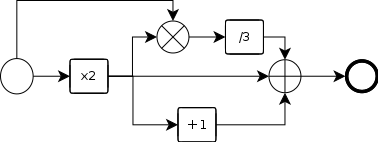
\includegraphics[scale=0.5]{./Figures/orchestration_example_diagram.png}
      \caption{Diagram}
    \end{subfigure}\\

    \begin{subfigure}[b]{.5\textwidth}
       \captionsetup{aboveskip=-5pt}
{\scriptsize
\begin{verbatim}  
FROM workflow: launching "f1"
FROM f1: input: 
data     sender   receiver 
2        init     f1       
4        init     f211     
FROM f1: selected input: 
data     sender   receiver 
2        init     f1       
FROM f1: processing

FROM workflow: launching "f2"
FROM f2: selected input: 
data     sender   receiver 
4        init     f211     
4        f1       f211     
4        f1       f22      

FROM f2: thread "f21" started
FROM f21: selected input: 
data     sender   receiver 
4        init     f211     
4        f1       f211     

FROM f21: launching "f211"
FROM f211: selected input: 
data     sender   receiver 
4        init     f211     
4        f1       f211     
FROM f211: processing

FROM f21: launching "f212"
FROM f212: selected input: 
data     sender   receiver 
16       f211     f212
FROM f212: processing
\end{verbatim}
  }
  \caption{Parts of \texttt{stdout}}
\end{subfigure}
\end{tabular}
\end{tabular}
\caption{Orchestration example}
\label{fig:orch_ex}
\end{figure*}
\subsection{Implementation of the framework}
To implement the framework with the orchestrator, we defined subclasses of QTask and QFunc for the specific processes.
\begin{itemize}
\item \textbf{QCreateDisk:} (inherits from QFunc, processed locally and sequentially) This function corresponds to the fork before PFE in figure \ref{fig:training}. It aims to create a disk with the dataset and all the code needed for selection.
  Its particular inputs are (here we will use a dictionary for multiple inputs).
  \begin{itemize}
  \item The qarnot connection (the concept is specific to the Qarnot SDK; a connection will define the building and home where the task will be scheduled)
  \item The directories of the files to put in the disk
  \item The labels of the data (alarm or not alarm)
  \item A disk (if a disk in given, this function only adds the code for selection)
  \item The local root of directories and the one the user wants them to be in the disk
  \end{itemize}
\item \textbf{QExtractFeaturesTask:} (inherits from QTask, processed on Q.rads and in parallel) This task corresponds to PFE in figure \ref{fig:training}. Given a disk of .wav file, a list of frame sizes and frame steps, this task separates the files in a number of portions and extracts features of each portion in parallel. The output is a disk containing .csv files with the features.
  Its particular attributes (in addition to those inherited from QTask) are
  \begin{itemize}
  \item The frame sizes and steps for extraction
  \item The remote root to find data
  \end{itemize}
\item \textbf{QLKOCVTask:} (inherits from QTask, processed on Q.rads and in parallel) This task corresponds to LKOCV in figure \ref{fig:training}. Given a disk of .csv features files, a list of parameters for grid search, this task aims to perform grid search in parallel. The process to make here consists of several parallel instance where each performs features integration (according to the parameters given) and a Leave-k-out cross validation on the dataset and writes in a file the false and true positive rates.
  Its particular attributes are
  \begin{itemize}
  \item The classification method (logistic regression, KNN, SVM)
  \item The length (in samples) of the data
  \item The remote root to find data
  \item The grid of parameters to test (parameters for extracting features and hyperparameters, the grid is created from both types of parameters)
  \item Other arguments for cross validation
  \end{itemize}
\item \textbf{QSelectionTask:} (inherits from QTask, processed on a Q.rad and sequentially i.e with only one parallel instance) This task corresponds to PSEL, EVAL and PSEL in figure \ref{fig:training}. It takes the results from QLKOCVTask and performs Pareto-selection to get the best classifiers on the training set. Then it tests these classifiers on the test set and performs Pareto-selection again to select the best classifiers. It returns the selected classifiers trained with all the dataset (train and test sets).
  Its particular attributes are
  \begin{itemize}
  \item The classification method
  \item The remote root to find data (train and test)
  \item Other arguments for Pareto selection
  \end{itemize}
\item \textbf{QDownloadResults:} (inherits from QFunc, processed locally and sequentially) This is to download the selected classifiers and the results.
\end{itemize}
\begin{figure}[H]
\centering
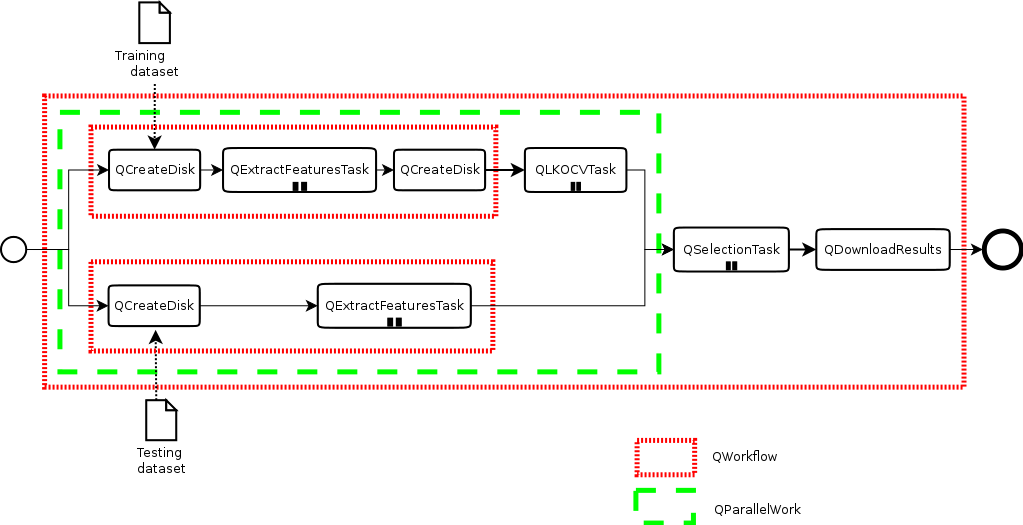
\includegraphics[width=0.5\textwidth]{Figures/implementation.png}
\caption{The proposed implementation of the framework using the orchestrator.}
\label{fig:implementation_diagram}
\end{figure}

Figures \ref{fig:implementation_diagram} and \ref{fig:implementation_code} show the implementation proposed for the framework of Figure~\ref{fig:training} in using the orchestrator. All basic blocs are created using the above subclasses and are combined using QWorkflow and QParallelWork. Note that we added a QCreateDisk after QExtractFeaturesTask to add the code needed for selection (this can be avoided by putting the code in the docker repository used for the tasks).

\begin{mdframed}[backgroundcolor=LightGray,topline=false, bottomline=false,leftline=false, rightline=false]
\inputminted[baselinestretch=1, fontsize=\scriptsize]{python}{selection.py}
\end{mdframed}
\captionof{figure}[belowskip=-20pt]{Source code of the proposed implementation.}
\label{fig:implementation_code}
\section{Experimental evaluation} \label{Proof-of-concept}
The implemented framework was tested using a database built using the method presented in figure \ref{fig:gen}. The alarm and the significant sounds (among which baby crying, laughs,power drill) were taken from the internet and ambiance sounds (office and talking) are $5s$ recordings of Qarnot Computing's office. We divided the ambiance sounds for training and testing sets and mixed them with the other sounds using different signal-to-noise ratio (SNR) to build the dataset. The dataset is presented in table \ref{table:dataset}.
\begin{table}[h]
  \centering
  \begin{tabular}{|*{3}{l|}}
    \hline
    & Training & Testing \\
    \hline
    \multicolumn{3}{|c|}{Background sounds} \\
    \hline
    office & 40 & 20\\
    talking & 100 & 50 \\
    \hline
    \multicolumn{3}{|c|}{Sounds of interest} \\
    \hline
    alarm & 1 & 1 \\
    others & 10 & 10 \\
    \hline
    \multicolumn{3}{|c|}{Mix} \\
    \hline
    SNR (dB)& -15,-5,0,5 & -20,-15,-10, -5,0,5 \\
    \hline
    \multicolumn{3}{|c|}{Total} \\ 
    \hline
    alarm & 560 & 420 \\
    non alarm & 5740 & 4270 \\
    total & 6300 & 4690 \\
   \hline
  \end{tabular}
\caption{dataset \label{table:dataset}}
\end{table}


\subsection{A feature centered view of the implemented framework} \label{subsec:extraction}
The features we used are defined in Figure \cite{pyAudioAnalysis}. 
Features are extracted on $K$ overlapping frames (called 'analysis frames') of the signal. A signal is then represented by $K$ vectors: $(x_k)_{k \in \iseg{0,K-1}}$ with $\forall k \in \iseg{0, K-1}, x_k \in \rset^d$ where $d$ is the number of features. These $K$ vectors are then integrated using several possible techniques. This integration means that we consider the sequence of features  $\left(x_{i,k}\right)_{k \in \iseg{0,K-1}}$ as a new signal which is cut in frames (called 'texture frames'). Then, some operations are done on these frames to aggregate the features \cite{DBLP:journals/taslp/JoderER09}. Classification is then performed on each vector of integrated features and a vote is done at the end to combine results (see figure \ref{fig:integration}). Note that the extraction part is done by a QExtractFeaturesTask and integration by a QLKOCVTask.
\begin{figure}[h]
  \captionsetup{belowskip=-10pt}
  \begin{center}
    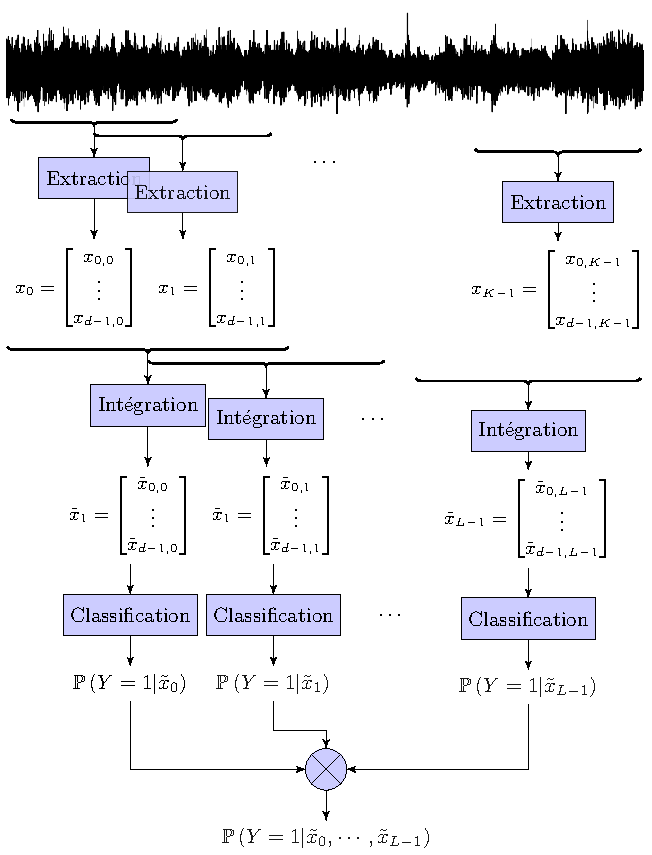
\includegraphics[width=0.3\textwidth]{Figures/integration.pdf}
  \end{center}
  \caption{Features extraction and integration \label{fig:integration}} 
\end{figure}

The features extraction was performed using the library \texttt{pyAudioAnalysis} \cite{pyAudioAnalysis} which implements well known features for audio signal processing such as Zero crossing rate, energy, spectral centroid and spread or MFCCs. A total of $d=34$ features were used. These features were extracted using several analysis frames sizes, integration methods ('stack' = concatenating all vectors, 'mVar' = concatenating mean and variance) and texture frames sizes. For analysis frames and textures frames we used an 50\% overlap. This features are referred as 'features parameters'. 
\subsection{Experimental setup}
The parameters we used for the grid search are of two sorts: features parameters (defined above) and hyperparameters (parameters of the classification method). We then ran the framework of Figure \ref{fig:implementation_diagram} to select for each classification technique the best combination of features parameters and hyperparameters. The list of all parameters used is presented in Table \ref{table:params}.

\begin{table}[h]
  \centering
  \begin{tabular}{|l|l|}
    \hline
    \multicolumn{2}{|c|}{Features parameters}                                          \\
      \hline
      Analysis frames size     & $2048, 4096, \cdots 65536, T$                         \\
      (in samples)             &                                                       \\
     \hline
     Integration               & None (if Analysis frames size = $T$),                 \\
                               & stack, mVar                                           \\
    \hline
    Texture frames size (in    & $4,8,16,32, \cdots,$ all                              \\
    number of analysis frames) &                                                       \\
    \hline
    \hline
    \multicolumn{2}{|c|}{Hyperparameters}                                              \\
     \hline
    Logistic regression        & $C \in \{0.1,1,10\}$                                  \\
    \hline
    KNN                        & $k \in \{5,10,15,\cdots,50\}$                         \\ 
    \hline
    \multirow{2}{*}{SVM}
                               & kernel $\in$ \{linear, gaussian\}                     \\
                               & $\gamma$ (for gaussian kernel) $\in \{1, 4, 16, 32\}$ \\       
  \hline

  \end{tabular}
\caption{list of parameters \label{table:params}}
\end{table}
\subsection{Classifier selection results}
We generated alarm sounds classifiers (with the SVM, KNN and logistic regression) in considering the workflow of 
Figure~\ref{fig:implementation_diagram}. 
The classification method which gave the best results is logistic regression with a FPR on the test set of $0.02$ and a TPR of $0.83$ (against for example FPR = $0.0007$ and TPR=$0.48$ for KNN and FPR=$0.24$ and TPR=$0.8$ for SVM). Figure \ref{fig:learning_curve} shows the learning curve for the selected classifier. This curve is encouraging since it corresponds to a high-variance situation in which increasing the size of the dataset is likely to give better results. This results shows that, used with the right classification method, the framework outputs accurate solutions. 
\begin{figure}[h]
  \centering
  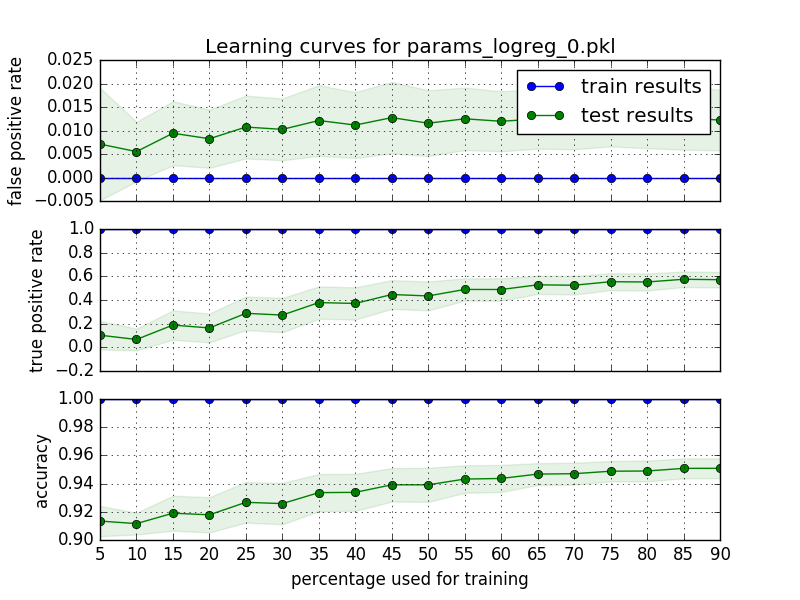
\includegraphics[width=0.4\textwidth]{Figures/learning_curve_logreg0_newdata.png}
  \caption{Learning curves for the best logistic regression classifier \label{fig:learning_curve}}
\end{figure}

\subsection{Runtime}
Here we present the runtime we obtained from runs of the workflow of Figure~\ref{fig:implementation_diagram} with the logistic 
regression method. The grid search in this cases visited a total of $129$ configurations. We did two series of experiments. 
The goal in the first serie was to find the best parallel granularity to run the workflow with. Indeed, 
QExtractFeaturesTask and QLKOCVTask can be done in parallel. A question is then to know how 
many parallel instances to run them with. We centered the search of the best granularity on the QLKOCVTask. 
Given $129$ configurations, we ran this process with $5, 10, 20$ and $129$ instances. For QExtractFeaturesTask,  
we used $10$ instances. This serie of experiments was done with a number of nodes (CPUs) equal to $34$. 

The second serie of experiment evaluates the scalability of the fine-grained solution (the number of parallel instance is equal to the 
number of configurations). Here we measure runtimes assuming that we want to find the best classifier from $25$,$50$,$100$ and $125$ 
configurations. In this serie, the number of nodes (CPUs) was equal to $25$ .  

Figure \ref{fig:times_extraction} shows the results for the extraction part which was ran with $10$ parallel instances for the train set and $10$ others for the test set (i.e $10$ parallel instances for each QExtractFeaturesTask). The first bar shows the time it would have taken to run the extraction sequentially (it is divided in two: the train set and the test set). The two other bars show the time it took to run QCreateDisk and QExtractFeaturesTask for both sets. The global time of the extraction in parallel is the time of the slowest instance i.e the one for train set which gives a global speedup of $1.9$. Figure \ref{fig:granularity} shows the results of granularity evaluation. The first observation is that the workflow does perform better than the sequential implementation. In subfigure \ref{subfig:granularity_ind}, are presented the individual runtime for QLKOCVTask and QSelectionTask. The main part of the workflow is QLKOCVTask and its runtime is reduced a lot by parallelism. On the contrary, the QSelectionTask would have performed better if it had been ran sequentially. The reason is simple: we implemented QSelectionTask as a sequential process which performs Pareto selection, evaluate the best classifiers on the test set and selects again. The reason we implemented it as a task is to simulate its behaviour on a Q.Rad. The difference between sequential and parallel times is due to loading times (the docker image, the data). However, this loss is not significant compared to the gain we get in QLKOCVTask.  Finally, in subfigure \ref{subfig:granularity_glob}, one can see that the speedup increases with the number of parallel instances and is at its maximum ($\approx 13$) for the finest granularity where there are as many instances as parameters. This behaviour made us believe that this fine-grained approach is the best and this is the reason why we tested scalability with this strategy. Figure \ref{fig:scalability} shows the results of this experiment. The main conclusion to have is that speedup increases with the number of parameters to test which is encouraging for scalability. However, the best scores show that testing more parameters is not always a good solution since they attain their optimum for 75 parameters. This question is inherently linked to the grid search strategy in which we decide to test all possibilities and will not be discussed here.

\setlength{\belowcaptionskip}{-6pt}
\setlength{\intextsep}{0pt}
\setlength{\textfloatsep}{1pt}

\begin{figure}
  \centering
  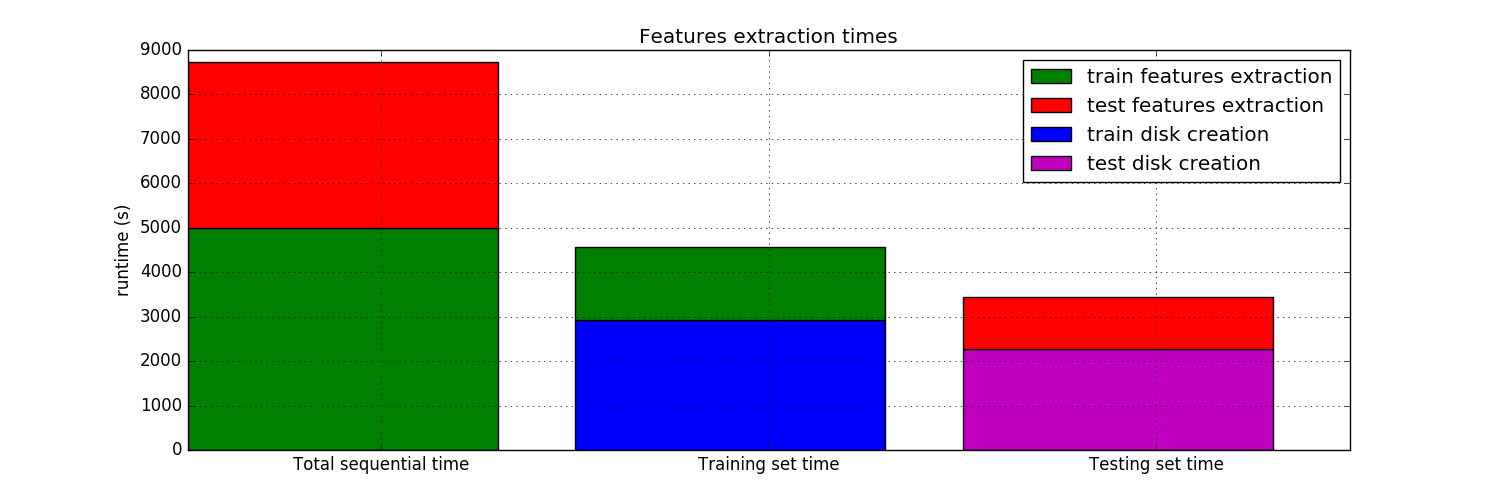
\includegraphics[width=0.5\textwidth]{Figures/times_extraction.png}
  \caption{Runtime for features extraction \label{fig:times_extraction}}
\end{figure}

\begin{figure}
  \begin{center}
    \begin{subfigure}{0.5\textwidth}
      \captionsetup{skip=0pt}
      \centering
      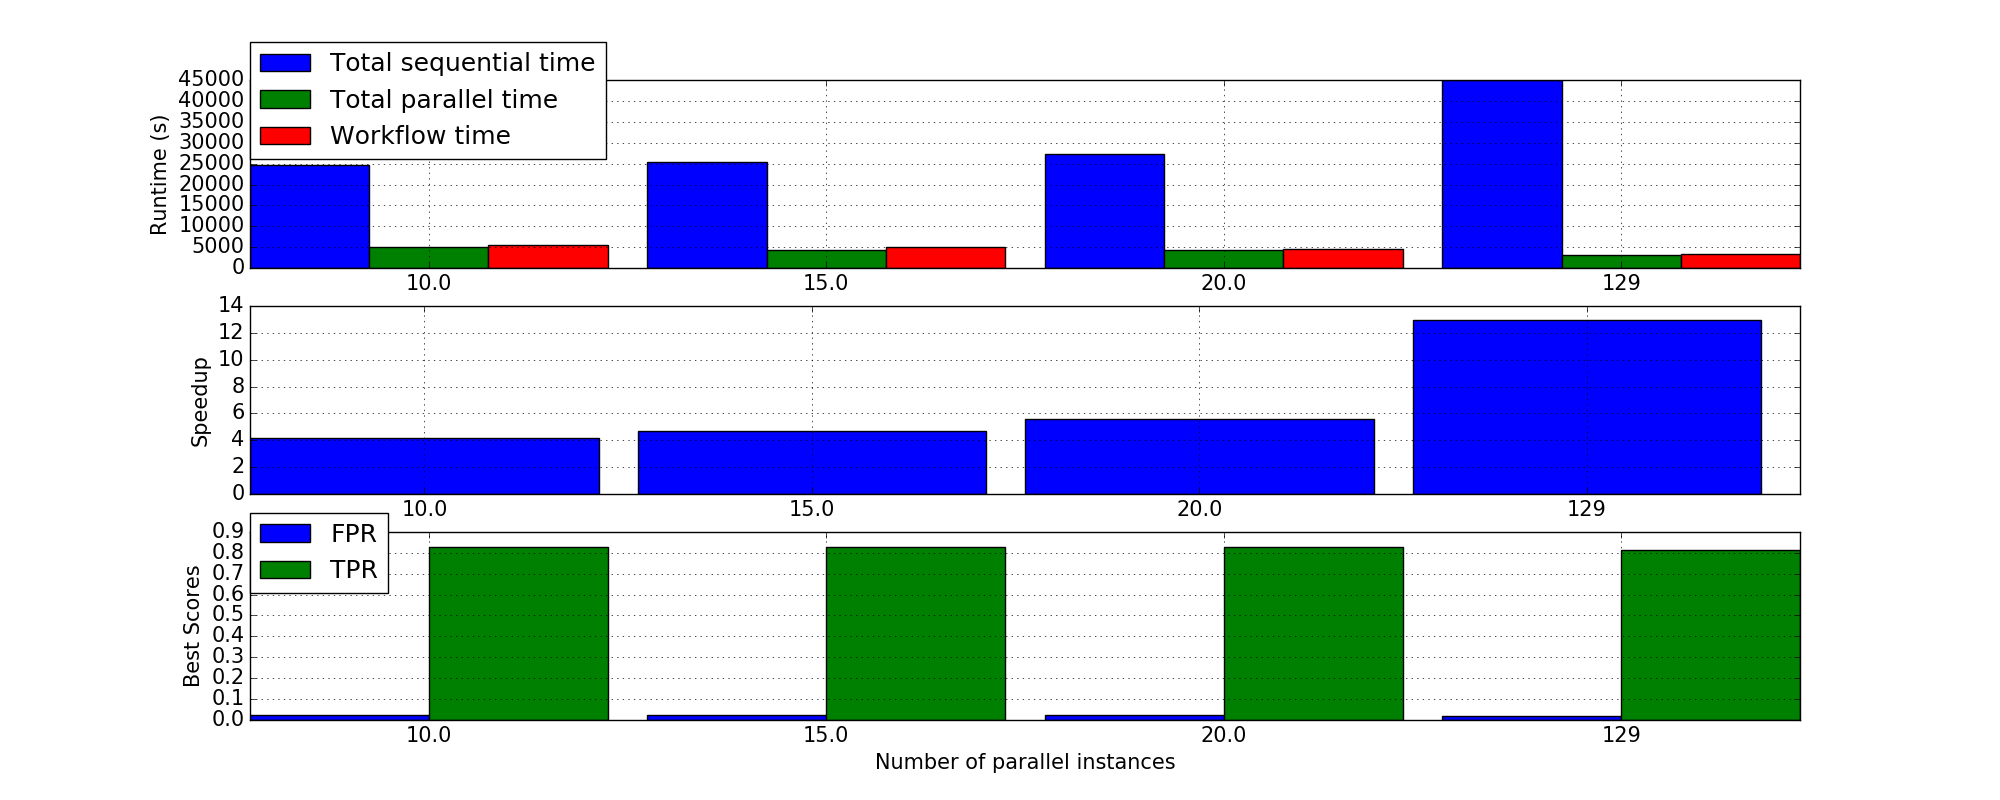
\includegraphics[width=\textwidth]{Figures/times_fixedparams_global_bars.png}
      \caption{\footnotesize Global results \label{subfig:granularity_glob}}
    \end{subfigure}\\
  \begin{subfigure}{0.5\textwidth}
    \captionsetup{skip=0pt}
    \centering
    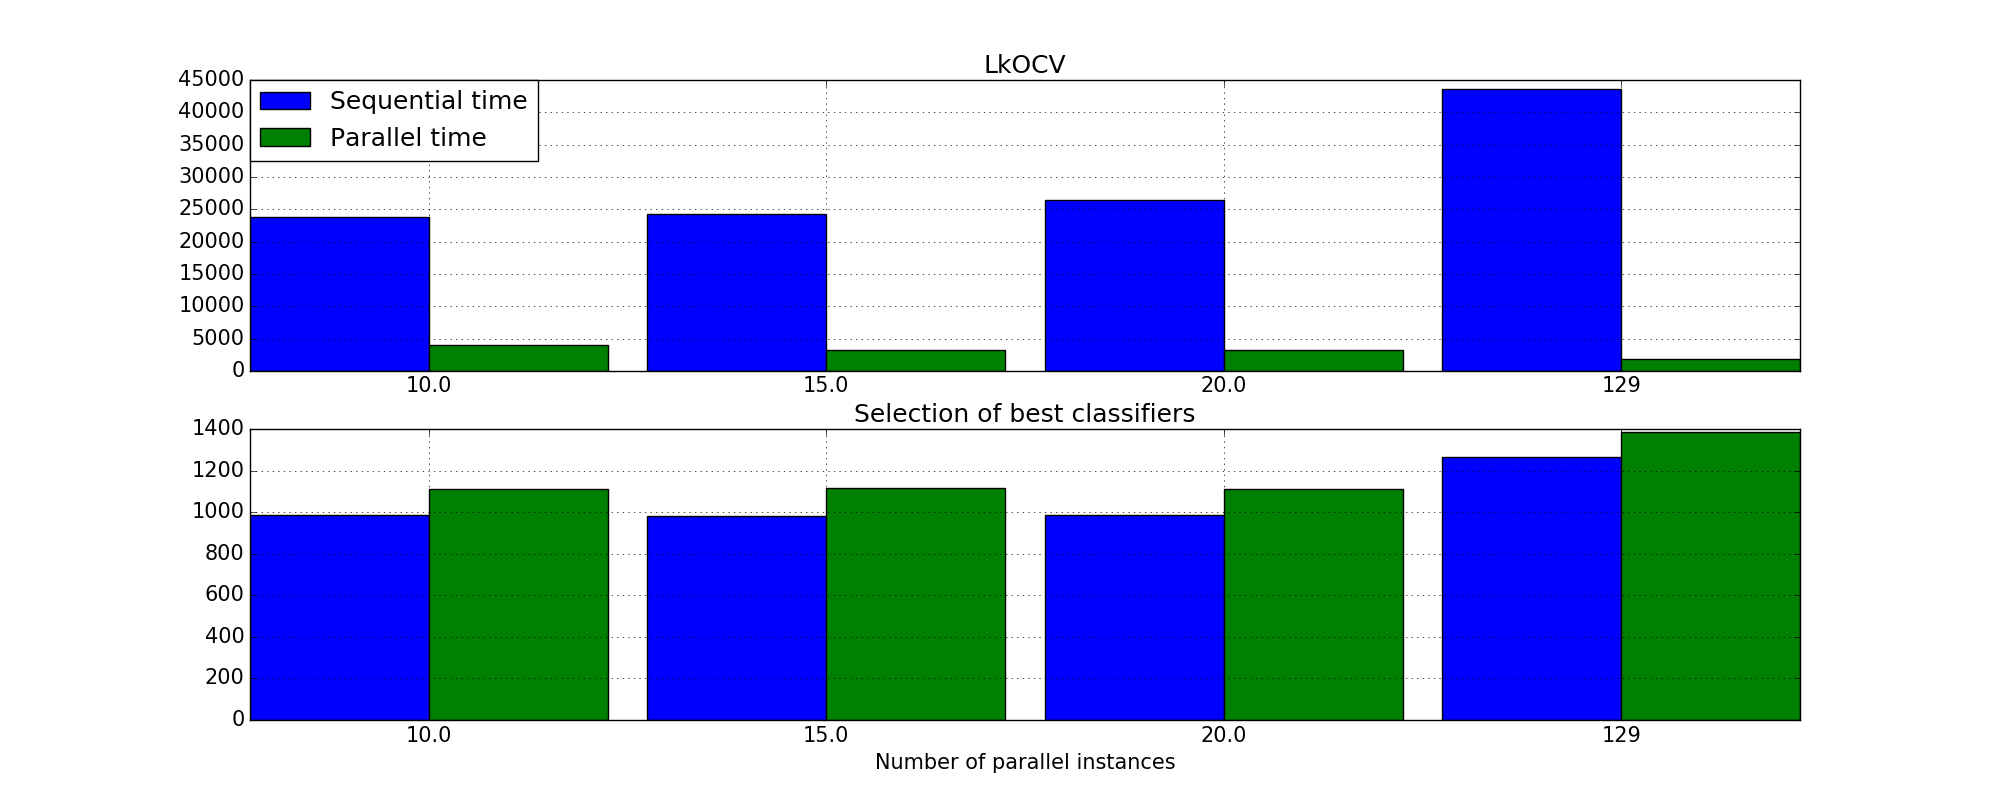
\includegraphics[width=\textwidth]{Figures/times_fixedparams_individual_bars.png}
    \caption{\footnotesize Individual tasks results \label{subfig:granularity_ind}}
  \end{subfigure}
\end{center}
\caption{Runtime for coarse-grained implementation \label{fig:granularity}}
\end{figure}

\begin{figure}[h]
  \begin{center}
    \begin{subfigure}{0.5\textwidth}
      \captionsetup{skip=0pt}
      \centering
      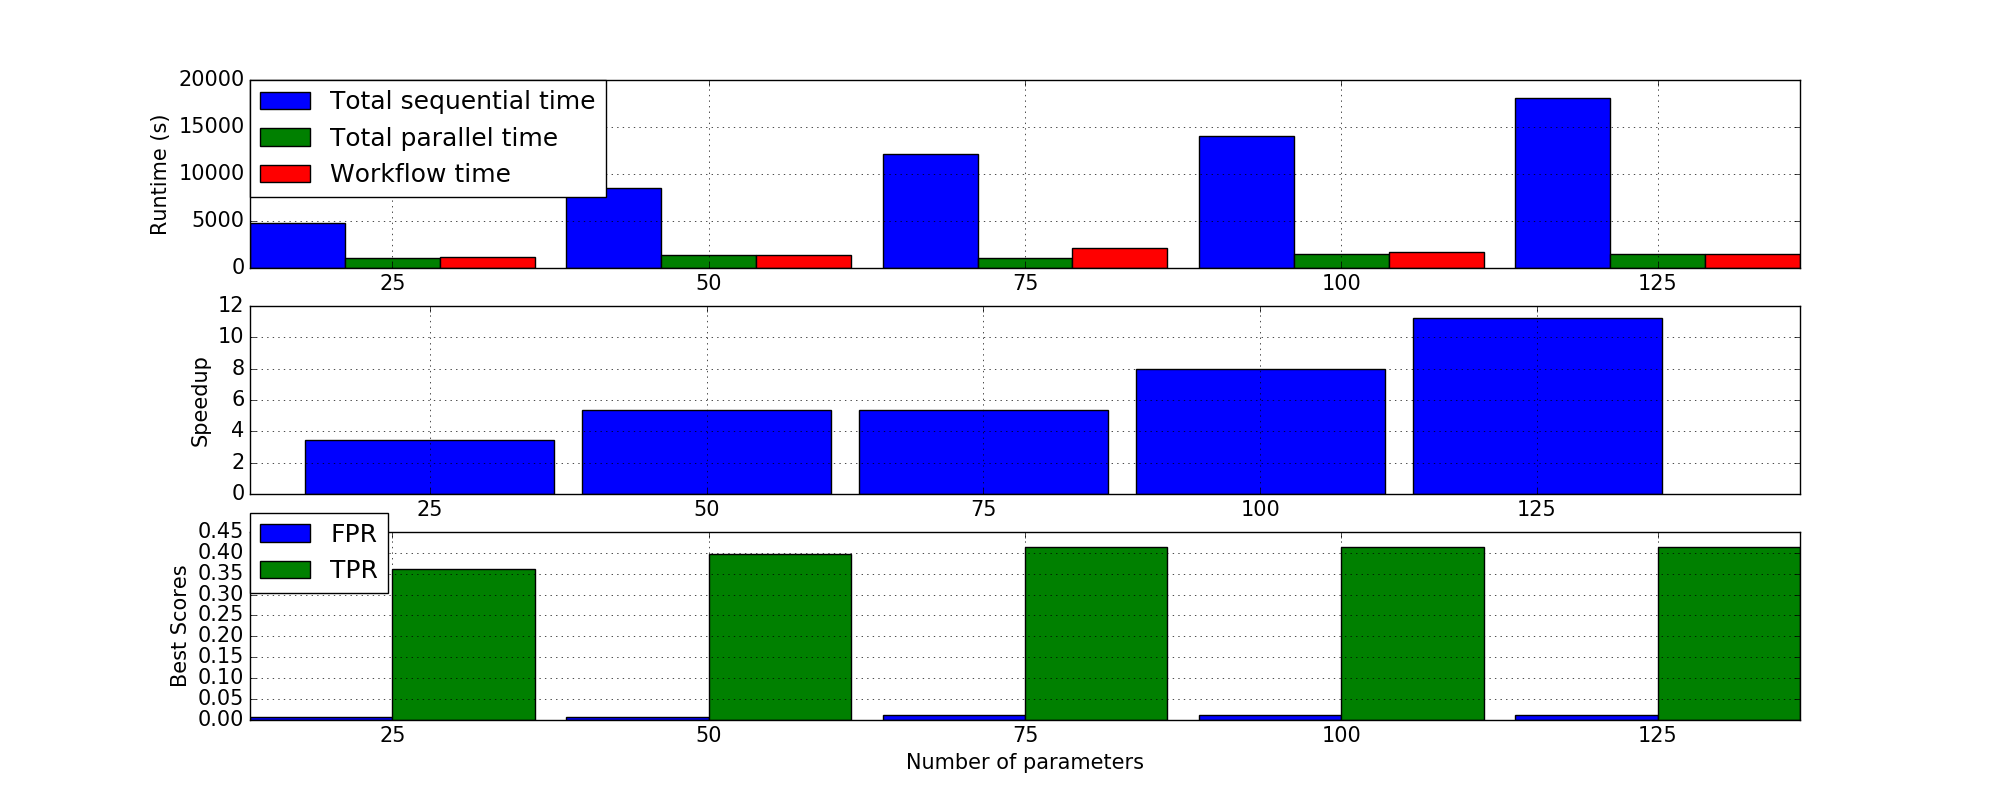
\includegraphics[width=\textwidth]{Figures/times_increasparams_global_bars.png}
      \caption{\footnotesize Global results \label{subfig:scalability_glob}}
  \end{subfigure} \\
  \begin{subfigure}{0.5\textwidth}
    \captionsetup{skip=0pt}
    \centering
    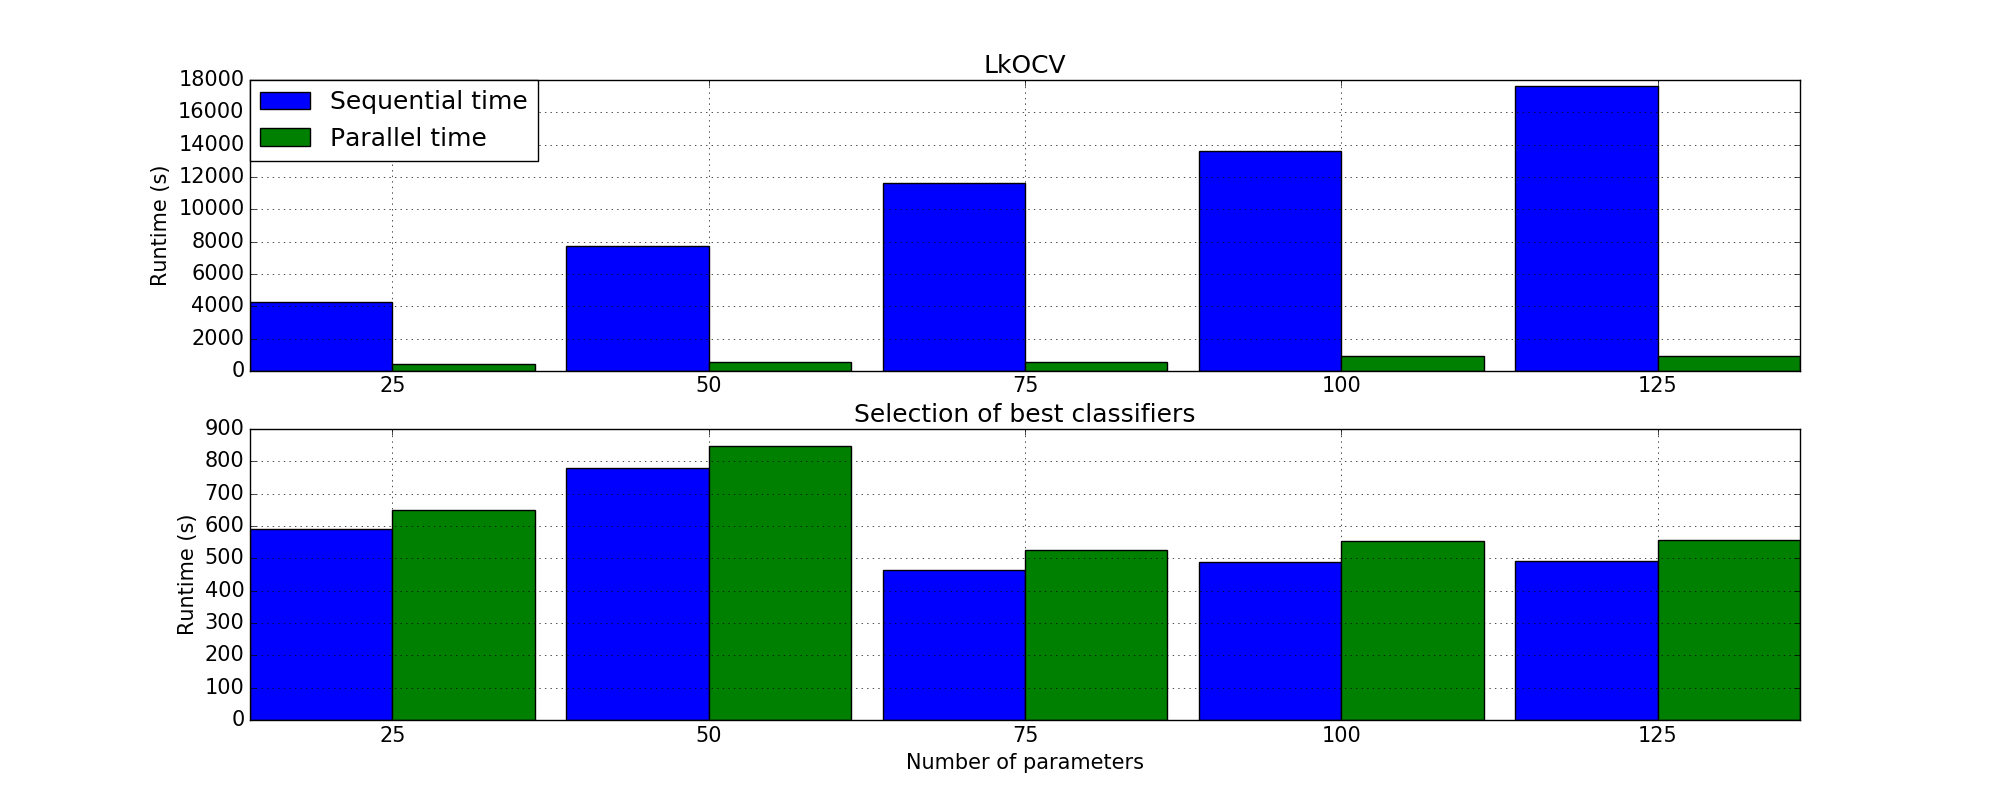
\includegraphics[width=\textwidth]{Figures/times_increasparams_individual_bars.png}
    \caption{\footnotesize Individual tasks results \label{subfig:scalability_ind}}
  \end{subfigure}
\end{center}
\caption{Runtime for fine-grained implementation \label{fig:scalability}}
\end{figure}
\section{Conclusion} \label{Conclusion}
The way Qarnot Computing performs computation is ideal for in-situ machine learning since collecting data and selecting the best classifier for the created dataset can be done within the same home or building. This leads to an improvement in terms of privacy and response time. We introduced an orchestration solution to create computing frameworks on this infrastructure. This orchestrator is intuitive since its components directly refer to graph elements and can model complex machine-learning frameworks such as classifier selection for alarm sounds detection. The strategy we proposed to solve this problem has shown good performances in term of accuracy of the outputs and scalability. However, the speedup obtained for features extraction could be increased by improving the infrastructure's data management mechanism.

\def\IEEEbibitemsep{.1pt}
\bibliographystyle{./IEEEtran}
\bibliography{acoustic}




% that's all folks

\end{document}

